% =================================================
% MAIN DOCUMENT (BOOK TEMPLATE)
% =================================================
%
% This file defines the logical and structural layout
% of the book.
%
% Typographic appearance is defined entirely in
% bookstyle.sty and should not be altered here.
%
% =================================================


% ENGINE: compile with LuaLaTeX, e.g.
%   latexmk -lualatex main.tex

% ------------------ Final print -------------------
\documentclass[12pt,twoside,b5paper]{book}

% ------------------ Draft / writing ---------------
% Same measure and line breaks as B5, with 4 cm
% margins for notes.
% \documentclass[12pt,twoside,a4paper]{book}


% =================================================
% LOAD BOOK STYLE
% =================================================
\usepackage{bookstyle}


% =================================================
% LANGUAGE
% =================================================
\usepackage[english]{babel}


% =================================================
% CUSTOM PACKAGES
%
% Add project-specific packages here.
% Do not insert packages elsewhere in the file.
% =================================================

\usepackage{amsmath}                 % mathematics
                                     % (no amssymb: unicode-math
                                     %  supplies the symbols)
\usepackage{graphicx}                % figures
\graphicspath{{figures/}}            % figures live in figures/
\usepackage{booktabs}                % tables


% =================================================
% CUSTOM COMMANDS
%
% Project-specific macros.
% =================================================

% \newcommand{\dd}{\mathrm{d}}
% \newcommand{\ii}{\mathrm{i}}


% =================================================
% DOCUMENT
% =================================================
\begin{document}


% =================================================
% FRONT MATTER
% =================================================
\frontmatter
\pagenumbering{roman}
\pagestyle{frontmatterstyle}


% ------------------ Title page -------------------
\title{Book Title}
\subtitle{An optional subtitle}
\author{Author Name}
\date{\the\year}

\booktitlepage
\thispagestyle{empty}


% ------------------ Blank verso ------------------
\clearpage
\null
\thispagestyle{empty}
\clearpage


% ------------------ Dedication -------------------
\dedicationpage{To someone.}


% ------------------ Table of contents ------------
\booktoc
\cleardoublepage


% ------------------ Preface ----------------------
\frontchapter{Preface}
\noindent
This is the preface to the book. It introduces the author's
motivation, intended audience, and approach. A preface speaks
in the author's own voice and is typically short --- two to
four pages.

A new paragraph continues the conversation. The preface is
where one might explain how the book came to be, what makes
this treatment different, and what assumptions are made of
the reader.

A book template uses placeholder text like this so the layout
can be inspected before any real writing begins. Replace this
text with your own preface.

\cleardoublepage


% ------------------ Acknowledgments --------------
\frontchapter{Acknowledgments}
\noindent
Acknowledgments are conventionally placed in the front matter,
just after the preface. They thank colleagues, institutions,
funding bodies, and family members who supported the work.

A short, sincere acknowledgment is generally preferred over an
exhaustive one. Two to four paragraphs is typical.

\cleardoublepage


% =================================================
% MAIN MATTER
% =================================================
\mainmatter
\pagestyle{chapterstyle}


% ------------------ Introduction -----------------
\chapter{Introduction}
\chapteropening{T}{his is the opening sentence}
of the introduction, set with a drop cap and small caps on
the first few words. The introduction lays out the structure
of the book, motivates the central questions, and previews
the arguments that will be developed in the chapters that
follow.

In a working manuscript, this chapter would survey the
landscape, define key terms, and set expectations for the
reader. It might end with a brief outline of the chapters
ahead --- a roadmap that orients the reader before they
encounter the technical material.


% ------------------ Part I -----------------------
\part{First Part}

\chapter{Chapter Title}
% Example chapter content.
% Replace with your own.

\chapteropening{T}{his is the opening sentence}
of the chapter, set with a drop cap and small caps on the
first few words. The opening paragraph should be long enough
to fill the vertical space reserved by the drop cap, otherwise
the next section heading will appear too close to it.

A second paragraph continues without extra spacing. Classical
book typography uses indented paragraphs and minimal vertical
white space --- the rhythm of the prose is what carries the
reader through.


\section{First Section}

A section heading without a number. The book template uses
unnumbered sections so that the chapter and part numbers
carry the structural hierarchy on their own. Sections still
appear in the table of contents, so navigation is preserved.

Citations in this template are rendered as small superscript
numbers, placed exactly where they belong in the text\cite{example-article}.
Multiple sources can be grouped within a single citation
and are sorted and compressed automatically\cite{example-article,example-book}.


\section{Mathematics}

Mathematics is set inline, $E = mc^2$, or as a numbered
display:
\begin{equation}
  i\hbar \frac{\partial \psi}{\partial t}
  = \hat{H}\psi.
  \label{eq:schrodinger}
\end{equation}
Equation \eqref{eq:schrodinger} is the time-dependent
Schr\"odinger equation, written here purely as an example
of a labeled display that can be referenced from elsewhere
in the chapter.

A second display can follow with a different label:
\begin{equation}
  \langle A \rangle_\psi = \langle \psi | \hat{A} | \psi \rangle.
  \label{eq:expectation}
\end{equation}
The spacing around displays is set in \texttt{bookstyle.sty}
and gives mathematics enough room to breathe without losing
contact with the surrounding text.

\subsection{A Subsection}

Subsections nest under sections and are also unnumbered.
They are useful when a section grows long enough to need
internal structure but not long enough to deserve its own
section.


\section{Figures and Tables}

A figure is included by placing the file in the \texttt{figures/}
folder and calling \texttt{\textbackslash includegraphics}:

\begin{figure}[t]
  \centering
  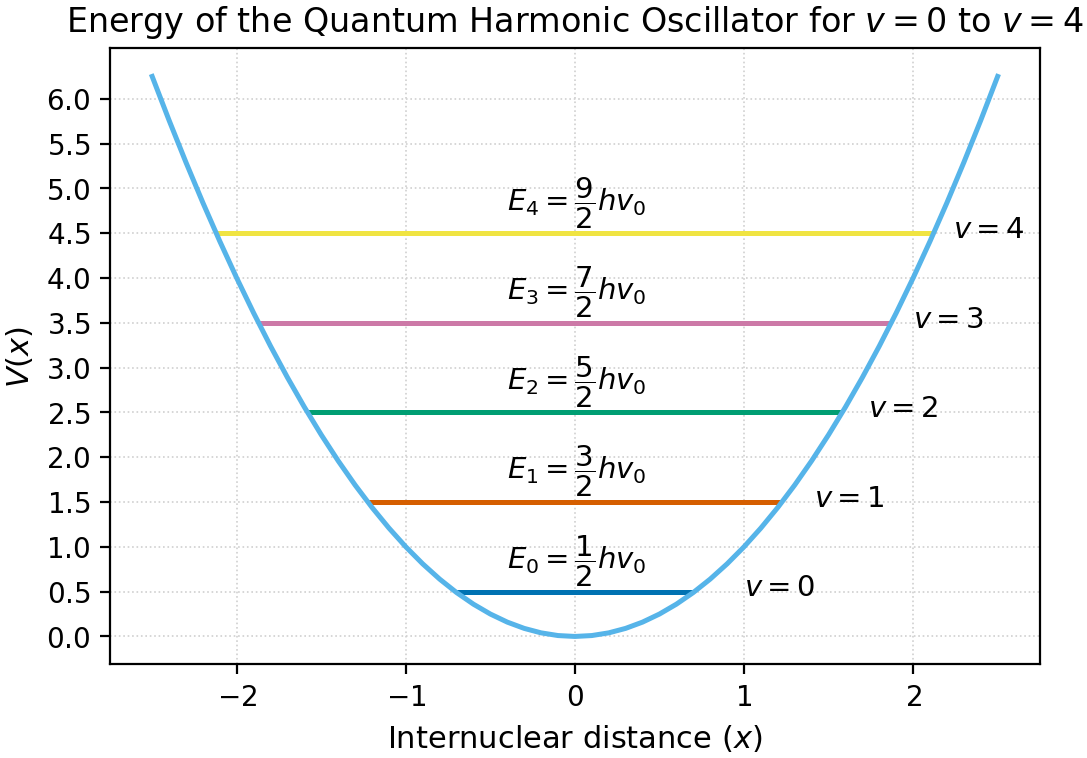
\includegraphics[width=0.7\linewidth]{Energy_levels}
  \caption{An example figure showing energy levels.}
  \label{fig:levels}
\end{figure}

Refer to figures with figure~\ref{fig:levels}. The float
placement \texttt{[t]} lets the figure rise to the top of a
page, which is the typical book convention --- figures rarely
sit inline in long-form prose.

A table can summarize key values:
\begin{table}[t]
  \centering
  \caption{Fundamental physical constants.}
  \label{tab:constants}
  \begin{tabular}{lcr}
    \toprule
    Quantity            & Symbol  & Value                         \\
    \midrule
    Speed of light      & $c$     & $2.998 \times 10^8$ m/s       \\
    Planck's constant   & $\hbar$ & $1.055 \times 10^{-34}$ Js    \\
    Elementary charge   & $e$     & $1.602 \times 10^{-19}$ C     \\
    \bottomrule
  \end{tabular}
\end{table}

% For native TikZ figures in a book, prefer the standalone workflow:
% compile each figure in its own file with \documentclass{standalone},
% then include the resulting PDF with \includegraphics.
% This keeps chapter files clean and avoids slow recompilation of the
% whole book when a figure changes.  The palette colors (darkred,
% darkorange, darkolive) defined in bookstyle.sty are available in
% standalone files via \usepackage{bookstyle} or \usepackage{xcolor}
% with the same \definecolor definitions.

Tables in this template use the \texttt{booktabs} convention:
horizontal rules only, used sparingly --- top, middle, and
bottom. Vertical lines are deliberately omitted.


\section{Closing}

A closing section can wrap up the chapter and gesture toward
the material in the next one. In a longer book, this is where
you might preview the next chapter or step back to summarize
what was covered.



% ------------------ Part II ----------------------
\part{Second Part}


% ------------------ Part III ---------------------
\part{Third Part}


% =================================================
% BACK MATTER
% =================================================
\backmatter

% ------------------ Bibliography -----------------
\bibliographystyle{unsrt}
\bibliography{references}

% ------------------ Index ------------------------
% \printindex


\end{document}
